\newcommand{\triangulationcomment}[1]{}

\chapter{2D Triangulations} \label{Chapter_2D_Triangulations}

\minitoc

This chapter describes the two dimensional triangulations
of \cgal. After a few definitions in 
section~\ref{Section_2D_Triangulations_Definitions}, 
the overall software
design of the 2D triangulation package is described 
in section~\ref{Section_2D_Triangulations_Software_Design}.
The next sections present the different two dimensional triangulations classes
available in  \cgal\ : 
basic triangulations (section~\ref{Section_2D_Triangulations_Basic}),
Delaunay triangulations
(section~\ref{Section_2D_Triangulations_Delaunay}),
regular triangulations
(section~\ref{Section_2D_Triangulations_Regular}),
constrained triangulations
(section~\ref{Section_2D_Triangulations_Constrained}),
and Delaunay constrained triangulations
(section~\ref{Section_2D_Triangulations_Constrained_Delaunay}).
At last, the section~\ref{Section_2D_Triangulations_Hierarchy}
described a hierarchical data structure for
fast point location queries.

\section{Definitions}
\label{Section_2D_Triangulations_Definitions}
A two-dimensional triangulation is a set $T$  of simplices of dimension 0,
1 or 2, called respectively vertices, edges and facets,
such that~: \\
- any face of a simplex in $T$ is a simplex in $T$ \\
- any simplex in $T$ is a face of a facet in $T$ \\
- two simplices in $T$ are either disjoints,
or incident (meaning that one is a subface of the other)
or they share a common lower dimensional face. \\
- the set of facets in  $T$ is connected for the adjacency relation,
 where two facets 
are said to be  {\em adjacent} if they
share a common edge.

Each facet of a triangulation can be given an orientation
which in turn induces an orientation
on the edges incident to that facet. The orientation of two adjacent
facets are said to be consistent if they induce
opposite orientations on their common incident edge.
A triangulation is said to be orientable if 
the orientation of each facet can be chosen in such a way
that all pairs of incident facets have consistent orientations. 
The two-dimensional triangulations represented in \cgal\
are orientable triangulations
embedded in a plane or in a higher dimensional space.

Strictly speaking, the term {\em face} should be used
to design  a face of any dimension,
and the two-dimensional faces of a triangulation 
should be properly called {\em facets}.
However, following a common usage, we hereafter often call {\em
faces}, the facets
of a two dimensional triangulation.




\section{Software Design}
\label{Section_2D_Triangulations_Software_Design}

Because a triangulation is merely a set of
triangular faces with constant-size complexity,
triangulations are not implemented
as a layer on top of a planar map.
\cgal\ uses a proper internal
representation of triangulations based on faces and vertices
rather than on edges. Such a  representation
saves storage space and results in faster
algorithms~ \cite{bdty-tcgal-00}.

Thus the basic elements of the representation are vertices and faces.
Each triangular face gives access to its three incident vertices 
and to its three adjacent faces. 
Each vertex gives access to one of its incident faces
and through that face to the circular list of its incident faces.
The edges are not explicitly represented, they are only represented 
through the adjacency relations of two faces.

\begin{figure}
\begin{ccTexOnly}
\begin{center}
\input{three_levels.ltex}
\end{center}
\end{ccTexOnly}
\caption{The three-layer design of triangulations.
\label{I1_Fig_three_levels}}
\begin{ccHtmlOnly}
<CENTER>
<img border=0 src=three_levels.gif align=center alt="Three_levels">
</CENTER>
\end{ccHtmlOnly}
\end{figure}


The triangulations in \cgal\ are represented
by a three-layer structure  analogous to the design used for polyhedral
surfaces, see Figure~\ref{I1_Fig_three_levels}. \\
The bottom layer is made of  the base classes for vertices and faces.
These base classes store some 
geometric informations such as the coordinate of vertices 
and any other attribute (such as a color, or boolean marks
for constrained edges etc.)
needed by the application.
The base classes handle
incidence and adjacency relations in term of \ccc{void*} pointers.
The use of \ccc{void*} pointers in the bottom layer 
makes easy 
the change of one of the base
classes, to deal with an extra attribute like a color for example.\\
The second layer is the \ccc{triangulation data structure}
which can be can be thought 
of as a container for faces and vertices
and takes care
of all the combinatorial aspects of the triangulation.
The {triangulation data structure} restores strong type checking,
implementing adjacency and incidence relations 
with type safe pointer operations.
For that purpose, the {triangulation data structure} defines its own face and vertex
classes which are derived
 from the corresponding 
base classes
so that geometric and additional information on vertices and faces 
are simply inherited. \\
  At last, the top layer, is  the \ccc{triangulation class}
which implements the user interface
and is responsible for the geometric embedding of the triangulation.
This class offers to the user
the high level functionalities that can be expected from a triangulation:
insertion  or removal of a vertex, traversal of the faces,
enumeration of the vertices,
traversal of the   faces incident to a given vertex, location of a given point etc.
The {triangulation class} defines its own 
vertex and face classes
derived from the corresponding class of the {triangulation data structure}.
The vertices and faces of the {triangulation class}
are only accessed through high levels concepts such as 
handles, iterators, or circulators,
according to the required functionalities of the access.
Being  responsible for the geometric embedding 
the triangulation class
comes in different flavors according to the kind of triangulation represented:
basic, Delaunay, regular, constrained or constrained Delaunay
 triangulations etc.

The triangulation classes of \cgal\ depend on two template parameters.
The first template parameter stands for
 a geometric traits class which is assumed to provide
the geometric objects (points, segments and triangles) 
forming  the triangulation and the geometric predicates on those objects.
The second template parameter stands for a model
of  triangulation data
structure acting as a container for faces and vertices
while  taking care of the combinatorial aspects of the triangulation. 
The triangulation data structure class is itself a template
class parametrized by the base classes for faces and vertices.


\section{Basic Triangulations}
\label{Section_2D_Triangulations_Basic}

\subsection{Description}
\label{Subsection_2D_Triangulations_Basic_Description}

The class \ccc{Triangulation_2<Traits,Tds>}
serves as a base class for all
planar embedded two-dimensional triangulations
in \cgal.
This class expects a model of  {geometric traits} class
as first template argument and a model of {triangulation data structure}
as second argument. The requirements  for the geometric traits
are described later in this section. 
The concept of 
{triangulation data structure} and some models for this concept are
described in chapter~\ref{Chapter_2D_Triangulation_Data_structure}.
\cgal\ provides a default for the triangulation data structure
template argument.
 
The class \ccc{Triangulation_2<Traits,Tds>}
is designed to represent triangulations
 of a sets of points in the plane.
Lets ${  A}$ be a planar set of points.  
A triangulation of the set ${  A}$ has vertices at the points of ${  A}$
and its domain covers the convex hull of ${  A}$.
It can be viewed as a planar partition of the plane
whose bounded faces are triangular and cover
the convex hull of ${  A}$. The single unbounded face of this partition
is the complementary of the convex hull of ${  A}$. 
In many applications, such as Kirkpatrick's hierarchy
or incremental Delaunay construction, it is convenient to
deal with only triangular faces. Therefore, we add to the
triangulation
a fictitious vertex, called the \ccc{infinite vertex}
and we make each  convex hull edge incident 
to an \ccc{infinite} 
face having as third vertex  the \ccc{infinite vertex}.
 In that way, each edge is incident to exactly two faces
and special cases at the
boundary of the convex hull are simpler to deal with.
In the following, we called {\it infinite}  the infinite vertex
and any face or edge 
incident  to the infinite vertex. Any face or edge non incident
to the infinite vertex as well as any vertex different from
the infinite vertex  is said to be {\it finite}.
Although it is convenient to draw a triangulation as in
figure~\ref{I1_Fig_infinite_vertex}, note that
the \ccc{infinite vertex} has no significant
coordinates and that no geometric predicate can be applied on it
or on an infinite face.

\begin{figure}
\begin{ccTexOnly}
\begin{center} \IpeScale{50} \Ipe{infinite_vertex.ipe} \end{center}
\end{ccTexOnly}
\caption{The infinite vertex.
\label{I1_Fig_infinite_vertex}}
\begin{ccHtmlOnly}
<CENTER>
<img border=0 src=infinite_vertex.gif align=center alt="Vertices at
infinity">
</CENTER>
\end{ccHtmlOnly}
\end{figure}

A triangulation is represented as a collection of vertices and faces that
are linked together through incidence and adjacency relations.
Each face gives access to its three incident vertices and to
its 
three adjacent faces. Each vertex gives access to one of its  incident
faces. 

The three vertices of a face are indexed with 0, 1 and 2
in counterclockwise order. The neighbor of a face are also 
indexed with 0,1,2 in such a way that the neighbor indexed by \ccc{i}
is opposite to the vertex with the same index.

The edges  are only implicitly represented
through the adjacency relations between their  two incident
faces. Each edge has two implicit representations : the edge
of a face \ccc{f}  which is opposed to the vertex indexed \ccc{i},
can be represented as well as an edge of the \ccc{neighbor(i)} of 
\ccc{f}.


Many of the classes in the triangulation package
offer  two functions \ccStyle{int cw(int i)} and 
\ccStyle{int ccw(int i)} 
which given the index of a vertex in a face
compute the index of the next vertex  of the same face
in clockwise
or counterclockwise order.
 Thus, for example the neighbor 
\ccc{neighbor(cw(i))} is
 the
neighbor of \ccc{f}  which is next to \ccc{neighbor(i)} turning clockwise
around \ccc{f}. The face \ccc{neighbor(cw(i))}
is also the first face encountered after \ccc{f} when
turning clockwise around vertex \ccc{i}
of~\ccc{f}. See Figure~\ref{I1_Fig_neighbors}.



 \begin{figure}
\begin{ccTexOnly}
    \begin{center}
     \input{neighbors.ltex}
    \end{center}
\end{ccTexOnly} 
    \caption{Vertices and neighbors.
    \label{I1_Fig_neighbors}}
  \begin{ccHtmlOnly}
<CENTER>
<img border=0 src=neighbors.gif align=center alt="Neighbors">
</CENTER>
\end{ccHtmlOnly} 
\end{figure}


The vertices and faces of the triangulations are accessed through 
\ccc{handles}\footnote{ A handle is a type which supports the two
dereference operators \ccc{operator*} and \ccc{operator->}.}, 
\ccc{iterators} and \ccc{circulators}. 
Handles are used whenever the accessed element 
is not part of a sequence,
iterators and circulators are used
to visit parts of the triangulation.

The triangulation class offers 
some iterators to visit all the (finite or infinite)
faces, edges or vertices and also iterators to visit all the finite
faces, edges  or vertices.
The triangulation offers circulators  
 to visit the edges or faces 
incident to a given vertex or the  vertices 
adjacent to it. It also provides a circulator type
to visit all the faces
traversed by a given line.
Circulators step through infinite features as well as 
through finite ones. 
The iterators and circulators
are all bidirectional and non mutable.
The circulators and iterators are assignable to the 
corresponding handle types. 
When calling a member function,
any handle type argument can be replaced
by an iterator or a circulator
with the same value type.

The triangulation class provides methods to test
the infinite character of any feature,
and also methods to test the presence in the triangulation
of a particular feature (edge or face) given its vertices.

The triangulation class  provides a method to locate
a given point with respect to a triangulation.
In particular, this method reports wether the point
coincides with a vertex of the triangulation, lies on an edge,
in a face or outside of the convex hull. In case of a degenerate 
lower dimensional triangulation, the query point may also lie
outside the triangulation affine hull.

The triangulation class also provides
methods to locate a point with respect to
a given  finite face of the triangulation or with respect to its
circumcircle.
The faces of the triangulation and their circimcircles 
have the  counterclockwise orientation.

The triangulation can be modified by several functions~:
insertion of a point, removal of a vertex,
flipping  of an edge. The flipping of an edge
is possible when the union of the two incident faces
forms  a convex body (see Figure~\ref{I1_fig_flip_bis}). 

\begin{figure}
\begin{ccTexOnly}
\begin{center} %\IpeScale{70} \Ipe{Flip.ipe} \end{center}
\input{flip.ltex}
\end{center}
\end{ccTexOnly} 
\caption{Flip. \label{I1_fig_flip_bis}}

\begin{ccHtmlOnly}
<CENTER>
<img border=0 src=Flip.gif align=center alt="Flip">
</CENTER>
\end{ccHtmlOnly} 
\end{figure}


\subsubsection{Implementation}

Locate is implemented by a line walk. The walk
begins  at  a vertex of the face which
is given
as an optional argument  or at an arbitrary vertex of the triangulation
 if no optional argument is given. It takes
time \ccTexHtml{$O(n)$}{O(n)} in the worst case, but only \ccTexHtml{$O(\sqrt{n})$}{O(sqrt(n))}
on average if the vertices are distributed uniformly at random.
The class \ccc{Triangulation_hierarchy_2<Traits,Tds>},
described in section~\ref{Section_2D_Triangulations_Hierarchy}, 
implements a data structure  designed to
offer an alternate  more efficient point location algorithm.

Insertion of a point is done by locating a face that contains the
point, and then splitting this face.
If the point falls outside the convex hull, the triangulation
 is restored by flips.  Apart from the location, insertion takes a
time \ccTexHtml{$O(1)$}{O(1)}. This bound is only an amortized bound
for points located outside the convex hull.

Removal of a vertex is done by removing all adjacent triangles, and
retriangulating the hole. Removal takes a time  at most proportionnal to
\ccTexHtml{$d^2$}{d^2}, where
 \ccTexHtml{$d$}{d} is the degree of the removed vertex,
which is \ccTexHtml{$O(1)$}{O(1)} for a random vertex.

The face, edge, and vertex iterators on finite features
are derived from their counterparts visiting all (finite and infinite)
features which are themselves derived from the corresponding iterators
of the triangulation data structure.


\subsubsection{ Geometric Traits}
\label{Subsubsection_2D_Triangulation_Basic_Geomrtric_Traits}

The first template parameter of the triangulation classes of \cgal\ 
is a geometric traits class. This parameter has to be instanciated by
a model of the concept
\ccc{TriangulationTraits_2} described \lcTex{
(\ccRefPage{TriangulationTraits_2})} of the reference manual.
 The geometric traits class 
is required to provide
the geometric objects (points, segments and triangles)
building up the triangulation
together with the geometric predicates on those objects.
The required predicates are: \\
- comparison of the \ccc{x} or \ccc{y} coordinates of two points.\\
- orientation tests providing \ccc{CGAL_orientation}
  corresponding to the order type of three given point.

The \cgal\  kernel classes \ccc{Homogeneous<Nt>} and
\ccc{Cartesian<Nt>},
templated by the number type \ccc{Nt} 
are models of the concept \ccc{TriangulationTraits_2}.

The \cgal\  library provides  other models
of \ccc{TriangulationTraits_2} 
using the kernel geometric objects and predicates.
These classes are themselves templated with a representation class. 
The traits class \ccc{Triangulation_euclidean_traits_2<R>}
is designed to deal with ordinary  two dimensional points.
The class \ccc{Triangulation_euclidean_traits_xy_3<R>} 
is a geometric traits class to build the triangulation
of a terrain. Such a triangulation is a two-dimensional
triangulation embedded  the three-dimensional space.
The data points are three-dimensional points.
The triangulation is 
build according to  the projections of those points
on the $xy$ plane  and then lifted up to the original
three-dimensional data points.
This is the usual case when dealing with GIS terrains.
Instead of really projecting the  three-dimensional points and
maintaining a mapping between each point and its projection
 (which costs space and is error prone),
the traits class  supplies geometric predicates that ignore the
\ccc{z}-coordinates of the points.
\cgal\ provides also the geometric traits classes
\ccc{Triangulation_euclidean_traits_yz_3<R>} and
\ccc{Triangulation_euclidean_traits_zx_3<R>} to
deal with projections on the
 \ccc{xz} plane  and  \ccc{yz}-plane,
respectively.

\subsection{Example of a Basic Triangulation}
\label{Subsection_2D_Triangulations_Basic_Example}

The following program  creates a  triangulation of 2D points
using the kernel model class \ccc{CGAL::Cartesian<double>}
as geometric traits and the default triangulation data structure
template parameter.
 The input points are read from a file 
and inserted in the triangulation.
Finally points on the convex hull are written to {\tt cout}. 
\ccIncludeExampleCode{Triangulation_2/triangulation_prog1.C}


\section{Delaunay Triangulations}
\label{Section_2D_Triangulations_Delaunay}

\subsection{Description}
\label{Subsection_2D_Triangulations_Delaunay_Description}
The class \ccc{Delaunay_triangulation_2<Traits,Tds>} is designed to represent
the Delaunay triangulation of a set of data points in the plane.
A  Delaunay triangulation of a set of points
fulfills
the following {\em empty circle property} 
(also called {\em Delaunay property}): the circumscribing
circle of any facets of the triangulation 
contains no data point in its interior.
For a point set with no subset of four cocircular points
the Delaunay triangulation is unique, it is  the dual
of the Voronoi diagram of the points.


A Delaunay triangulation is a special triangulation of a set of points.
So it is natural to derive  
the class \ccc{Delaunay_triangulation_2<Traits,Tds>}
from the basic class \ccc{Triangulation_2<Traits,Tds>}.
Like its base class, the Delaunay triangulation class is parametrized
by  two template 
parameters,  the geometric traits \ccc{Traits}
and the triangulation data structure\ccc{Tds}.
Just like the triangulation  data structure
of a basic triangulation,
the triangulation data strucure  of a Delaunay triangulation
has to be a   model of the concept \ccc{TriangulationDataStructure_2}.
In contrast, because the
concept of Delaunay triangulation relies on the notions of
distance and  
empty circles, 
the geometric traits has to be a model of the concept
\ccc{DelaunayTriangulationTraits_2}
which refines the concept \ccc{TriangulationTraits_2}.




The class \ccc{Delaunay_triangulation_2<Traits,Tds>}
inherits the types defined by the 
basic class \ccc{Triangulation_2<Traits,Tds>}.
Additionnal types, provided by the traits class,
are defined to represent the dual Voronoi diagram.


The class \ccc{Delaunay_triangulation_2<Traits,Tds>}
overwrite the member functions that insert a new point
in the triangulation or
or remove a vertex  from it
to maintain the Delaunay property.
It also has a member function (\ccc{Vertex_handle
        nearest_vertex(const Point& p)})
to answer nearest neighbor queries
and member functions to construct the elements (vertices and edges)
of the dual Voronoi diagram.

\ccHeading{Geometric traits}
The geometric traits has to be a model of the concept
\ccc{DelaunayTriangulationTraits_2}
which refines the concept \ccc{TriangulationTraits_2}.
In particular this concept provides
the \ccc{in_circle(p,q,r,s)} predicate
which decides the position of  the point $s$ (interior, exterior
or on the boundary) with respect to the circle
passing through $p$, $q$ and $r$. 
The \ccc{in_circle(p,q,r,s)}
predicate actually defines the Delaunay triangulation.
Changing this predicate 
allows to build Delaunay triangulations for different metrics
such that $L_1$ or $L_{\infty}$ or any metric defined by a
convex object. However, the user of an exotic metric
must be carefull that the constructed triangulation 
has to be a triangulation of the convex hull
which means that convex hull edges have to be Delaunay edges.
This is granted for any smooth convex metric (like $L_2$)
and can be ensured for other metrics (like  $L_{\infty}$)
by the addition to the point set of well chosen sentinel points.

The \cgal\  kernel classes \ccc{Homogeneous<Nt>} and
\ccc{Cartesian<Nt>}, and the class \ccc{Triangulation_euclidean_traits_2<R>}
are models of the concept \ccc{DelaunayTriangulationTraits_2}
for the euclidean metric.
\cgal\  also  provides traits classes to deal with terrains,
that are  two dimensional triangulated surfaces
embedded in the three  dimensional space that have project on 
a two dimensional  Delaunay triangulation. Namely, the traits classes
\ccc{Triangulation_euclidean_traits_xy_3<R>},\\
\ccc{Triangulation_euclidean_traits_yz_3<R>}, and\\
\ccc{Triangulation_euclidean_traits_zx_3<R>} \\
are to be used to build a a triangulated surface
projecting on the Delaunay triangulation of respectively
the \ccc{xy}, \ccc{yz} or \ccc{zx} projections of its vertices:\\
The requirements for the duality functions and nearest vertex
queries are not yet satisfied by
these last three classes.

\ccHeading{Implementation}
The insertion of a new point in the Delaunay triangulation
is performed using first the insertion member function
of the basic triangulation and second 
performing a sequence of flips to restore the Delaunay property. 
The number of flips that have to be performed is \ccTexHtml{$O(d)$}{O(d)}
if the new vertex has degree \ccTexHtml{$d$}{d} in the updated
Delaunay triangulation. For
points distributed uniformly at random, 
each insertion takes time \ccTexHtml{$O(1)$}{O(1)} on
average, once the point has benn located in the triangulation.

Removal calls the removal in the triangulation and then retriangulates
the hole created in such a way that  the Delaunay criterion is
satisfied. Removal of a
vertex of degree \ccTexHtml{$d$}{d} takes time \ccTexHtml{$O(d^2)$}{O(d^2)}.
The degree $d$ is \ccTexHtml{$O(1)$}{O(1)} for a random
vertex in the triangulation.

After having performed a  point location, the
nearest neighbor of a point is found in time \ccTexHtml{$O(n)$}{O(n)} in the
worst case, but in time \ccTexHtml{$O(1)$}{O(1)}
for vertices distributed uniformly at random  and any query point. 


\subsection{Example : a Delaunay Terrain}
\label{Subsection_2D_Triangulations_Delaunay_Terrain}

The following code  creates a Delaunay triangulation with 
the usual Euclidean metric for the vertical projection of a 
terrain model. The points have elevation, that is they are 3D points,
but the predicates used to build the  Delaunay triangulation
are computed using only  the $x$ and $y$ coordinates  
of these points. 
\ccIncludeExampleCode{Triangulation_2/terrain.C}

\subsection{Example : Voronoi Diagram}
\label{Subsection_2D_Triangulations_Voronoi}
\ccIndexMainItem{Voronoi diagram}
The following code computes the edges of Voronoi diagram
of a set of data points
and counts  the number of finite edges and the number of rays
of this diagram
\ccIncludeExampleCode{Triangulation_2/voronoi.C}


\section{Regular triangulations}
\label{Section_2D_Triangulations_Regular}

\subsection{Description}
\label{Subsection_2D_Triangulations_Regular_Description}
\ccIndexMainItem{power diagram}
Let ${  PW} = \{(p_i, w_i), i = 1, \ldots , n \}$ be a set of 
weighted points where each $p_i$ is a point and each $w_i$
is a scalar called the weight of point $p_i$.
Alternatively, each weighted point $(p_i, w_i)$ can be regarded
as a sphere (or a circle, depending on the dimensionality
of $p_i$)  with center $p_i$ and radius $r_i=\sqrt{w_i}$.

The power diagram of the set ${  PW}$ is a space partition in which
 each cell corresponds to a sphere $(p_i, w_i)$ of ${  PW}$
and is the locus of points  $p$ whose power with respect to $(p_i, w_i)$
is less than its power with respect to any other sphere 
in ${  PW}$. In the two-dimensional space,
the dual of this diagram is a triangulation 
whose domain covers the convex hull of the set 
${  P}= \{ p_i, i = 1, \ldots , n \}$ of center points
and whose vertices form a subset of ${  P}$.
Such a triangulation is called a regular triangulation.
Three points $p_i, p_j$ and $p_k$ of ${  P}$
form a triangle in the regular triangulation of ${  PW}$
iff there is a point $p$ of the plane with equal 
powers with respect to $(p_i, w_i)$, $(p_j, w_j)$
and $(p_k, w_k)$ and such that this power 
is  less than the power of $p$
with respect to any other sphere in  ${  PW}$.

Let us defined the power product of two weighted points
$(p_i, w_i)$ and $(p_j, w_j)$ as:
\[\Pi(p_i, w_i,p_j, w_j) = p_ip_j ^2 - w_i  - w_j  .\]
$\Pi(p_i, w_i,p_j, 0)$ is simply the power of point $p_j$
with respect to the sphere $(p_i, w_i)$, and two weighted points 
are said to be orthogonal if their power product is null.
The power circle of three weighted points
 $(p_i, w_i)$, $(p_j, w_j)$
and $(p_k, w_k)$ is defined as the unique circle
$(\pi, \omega)$  orthogonal to
 $(p_i, w_i)$, $(p_j, w_j)$
and $(p_k, w_k)$.

The regular triangulation of the sets ${  PW}$
satisfies the following {\em regular property} (which just reduces to the 
Delaunay property when all the weights are null):
a triangle $p_ip_jp_k$ is a face of the regular triangulation
of ${  PW}$ iff the power product of any weighted point
 $(p_l, w_l)$ of ${  PW}$ with the power circle of
 $(p_i, w_i)$, $(p_j, w_j)$ and $(p_k, w_k)$ is positive or null.
We call  power test of  $(p_i, w_i)$, $(p_j, w_j)$, $(p_k, w_k)$,
and $(p_l, w_l)$,  the predicates which amount to compute
the sign of 
the power product of $(p_l, w_l)$ with respect to
the power circle of
 $(p_i, w_i)$, $(p_j, w_j)$ and $(p_k, w_k)$.
This predicate amounts to computing the sign of
the following
determinant
\[\left| \begin{array}{cccc}
1  &  x_i  &  y_i  &  x_i ^2 + y_i ^2 - w_i  \\
1  &  x_j  &  y_j  &  x_j ^2 + y_j ^2 - w_j  \\
1  &  x_k  &  y_k  &  x_k ^2 + y_k ^2 - w_k  \\
1  &  x_l  &  y_l  &  x_l ^2 + y_l ^2 - w_l
\end{array}
\right|
\]

A pair of neighboring faces $p_ip_jp_k$
and $p_ip_jp_l$ is said to be locally regular
(with respect to  the weights in ${  PW}$)
if the power test of $(p_i, w_i)$, $(p_j, w_j)$, $(p_k, w_k)$,
and $(p_l, w_l)$ is positive.
A classical  result of computational geometry
establishes that a triangulation of the convex hull of ${  P}$
such that any pair of neighboring faces is regular with respect
to ${  PW}$, is a
 regular triangulation of ${  PW}$.

Alternatively, the regular triangulation
of the weighted points set ${  PW}$
can be obtained as the projection
on the two dimensional plane of the convex hull of the set of three
dimensional points 
${  P'}= \{ (p_i,p_i ^2 - w_i ), i = 1, \ldots , n \}$.

The class \ccc{Regular_triangulation_2<Traits, Tds>}
 is designed to maintain the
regular triangulation of a set of $2d$ weighted points.
The template parameters \ccc{Traits}  and \ccc{Tds} stand respectively
 for a geometric traits class and a triangulation data structure class.
The triangulation data structure has to be a model of the concept
\ccc{TriangulationDataStructure_2}.
The geometric traits class must provide a weighted point type
and a power test on these weighted points
and the concept for this parameter, called
\ccc{RegularTriangulationTraits_2},
is a refinement of the concept
\ccc{TriangulationTraits_2}. \cgal\ provides 
the class
\ccc{Regular_triangulation_euclidean_traits_2<Rep,Weight>}
which is a model for the traits concept
\ccc{RegularTriangulationTraits_2}.
The class \ccc{Regular_triangulation_euclidean_traits_2<Rep,Weight>}
derives  from the class
\ccc{Triangulation_euclidean_traits_2<Rep>}
and uses a \ccc{Weighted_point} type
derived from the type \ccc{Point_2} of
\ccc{Triangulation_euclidean_traits_2<Rep>}.


The class \ccc{Regular_triangulation_2<Traits, Tds>}
derives from the class \ccc{Triangulation_2<Traits, Tds>}.
The functions \ccc{insert} and 
\ccc{remove} are overwritten to maintain the regular
property.
The vertices of the regular triangulation
of a set of weighted points ${  PW}$ form only a subset
of the set of center points of ${   PW}$.
Some of the input
weigthed points have no cell in the dual power diagrams
and therefore do not correspond to a vertex of the regular
triangulation.
Therefore the  insertion of a weighted point  in a regular triangulation
does not necessarily imply the creation of a new vertex.

Regular triangulation have member functions to construct
the vertices and edges of the dual power diagrams.


\subsubsection{The Face Type of a Regular Triangulation}

An input  point that does not appear as a vertex in the
regular triangulation is said to be {\it hidden }
by the face in which the corresponding center point is located.
A  point which is hidden at a given time may appear later as a vertex of
the regular triangulation if some other weighted points are removed.
Therefore, hidden points have to be stored somewhere.
A hidden point can appear as vertex of the triangulation
only when the
two dimensional face that hides it
is removed from the triangulation. 
Therefore the  hidden point are stored
in the faces that  hide them and the nested face type of a 
regular triangulation is assumed to include a list of hidden 
weighted points. This list of weighted point is in fact included
in the base face of a regular triangulation.

Therefore the base face type of a regular triangulation
is required to provide a list of weigthed points,
designed to store the points hidden by the face. It has to be a model
of the concept \ccc{RegularTriangulationFaceBase_2}.
\cgal\ provides the templated class 
\ccc{Regular_triangulation_face_base_2<Traits>}
as a default base class for faces of regular triangulations.
This class  derives from \ccc{Triangulation_face_base_2<Traits>}.


\subsection{Example : a Regular Triangulation}
\label{Subsection_2D_Triangulations_Regular_Example}

The following code  creates a regular triangulation 
of a set of weighted points.

\ccIncludeExampleCode{Triangulation_2/regular.C}


\section{Constrained Triangulations}
\label{Section_2D_Triangulations_Constrained}

%\subsection{Description}
\label{Subsection_2D_Triangulations_Constrained_Description}
A constrained triangulation is a triangulation of a set of points
that has to include among its edges 
a given set of segments joining the points. The corresponding 
edges are called {\em constrained edges}. 

The endpoints of constrained edges are of course vertices of the
triangulation. However the triangulation may include
include other vertices as well.  The set of
constrained edges forms a set of segments that do not intersect
except possibly at their endpoints.  Any number of constrained edges
are allowed to share the same endpoint.  Vertical constrained edges or
constrained edges with null length are allowed.

\begin{ccTexOnly}
\begin{center} \IpeScale{50} \Ipe{constraints.ipe} \end{center}
\end{ccTexOnly}
 
\begin{ccHtmlOnly}
<CENTER>
<img border=0 src=constraints.gif align=center alt="A set of
constraints and its constrained triangulation">
</CENTER>
\end{ccHtmlOnly}

A constrained triangulation is represented in the CGAL library as an
object of the class \ccc{Constrained_triangulation_2<Traits,Tds>}.
The template parameter \ccc{Traits} 
stands for a geometric traits class  that has to be a model
of the concept \ccc{TriangulationTraits_2}.
The template parameter \ccc{Tds}
stands for 
a triangulation data structure class that has to be a model
of the concept \ccc{TriangulationDataStructure_2}.

The class \ccc{Constrained_triangulation_2<Traits,Tds>}
inherits from \ccc{Triangulation_2<Traits,Tds>}.
It defines an additionnal type \ccc{Constraint}
to represent the constraints. A
constraint is represented as a pair of points.

A  constrained triangulation can be created
from a
list of constrained edges.
The class \ccc{Constrained_triangulation_2<Traits,Tds>}
overrides the insertion and removal of a point to take care of the
information about constrained edges. The class also allows inline
insertion of a new constraint, given by its two endpoints
or the removal of a constraint.

\subsubsection{The Base Face of a Constrained Triangulation}
 The information about constrained edges is store in the 
faces of the triangulation. Thus the nested \ccc{Face}
type of a constrained triangulation offers
additonnal functionalities to deal with this information.
To achieve this, the base face of a Constrained Triangulation
has to be a model for the concept \ccc{ConstrainedFaceBase_2}
which refines the concept \ccc{TriangulationFaceBase_2}.
The concept \ccc{ConstrainedFaceBase_2}
requires  a member function
(\ccc{bool is_constrained(int i)})
 providing the status
(constrained ou unconstrained) of the edges
and also a member function 
(\ccc{void  set_constraint(int i, bool b)}) to set this status.


\cgal\ provides a default base face class
for constrained triangulations. This class, named
\ccc{Constrained_triangulation_face_base_2<Traits>},
derives from the class
\ccc{Triangulation_face_base_2<Traits>}
and add three boolean to store the status of its edges. 

%\subsubsection{A Constrained Triangulation Class for Animation Purposes
%\cgal\ provides 
%a class  \ccc{Constrained_triangulation_demo_2<Traits,Tds>}
%specially designed to show an animation of the sweep algorithm 
%that builds a 
%constrained triangulation from a list of constraints.

\begin{figure}
\begin{ccTexOnly}
\begin{center}
\includegraphics[width=6cm]{poisson.ps}
\includegraphics[width=6cm]{del_poisson.ps}
\end{center}
\end{ccTexOnly}
\caption{Constrained and Constrained Delaunay triangulation : 
 the constraining edges are the green edges,  a constrained
triangulation is shown on the left, the constrained Delaunay
triangulation with two examples of circumcircles is shown on the right.}
\label{I1_Fig_constrained}
\begin{ccHtmlOnly}
<CENTER>
<img border=0 src=poisson.gif alt=" Constrained triangulation">
<img border=0 src=del_poisson.gif alt="Constrained Delaunay triangulation">
</CENTER>
\end{ccHtmlOnly}
\end{figure}


\section{Constrained Delaunay Triangulations}
\label{Section_2D_Triangulations_Constrained_Delaunay}

%\subsection{Description}
\label{Subsection_2D_Triangulations_Constrained_Delaunay_Description}
A constrained Delaunay triangulation is a triangulation with
constrained edges which tries to be as much Delaunay as possible.
As constrained edges are not necessarily Delaunay edges,
the triangles of a constrained Delaunay triangulation do not
necessarily fulfill the empty circle property
but they fulfill a weaker \ccc{constrained empty circle property}.
 To state this property,
it is convenient to think of  constrained
edges as blocking the view. Then, a triangulation is 
constrained Delaunay iff
 the circumscribing circle
of any facets encloses 
no vertex  visible
from the interior of the facet.

The \cgal\ class
\ccc{Constrained_Delaunay_triangulation_2<Traits,Tds>}
is designed to represent
constrained Delaunay triangulations.

The class is templated by a geometric traits class \ccc{Traits}
and a triangulation data structure \ccc{Tds}.
The triangulation data structure has to be a model of the concept
\ccc{TriangulationDataStructure_2}.
 The geometric traits 
of a constrained Delaunay triangulation is required
to provide the \ccc{side_of_oriented_circle} test as the geometric traits
of a Delaunay triangulation and has to a model of the concept
\ccc{DelaunayTriangulationTraits_2}.

A constrained Delaunay triangulation is not a Delaunay
triangulation but it is a constrained triangulation.
Therefore the class
\ccc{Constrained_Delaunay_triangulation_2<Traits,Tds>}
derives from
the class \ccc{Constrained_triangulation_2<Traits,Tds>}.
Also, information about the status (constrained or not)
of the edges of the triangulation has to be stored
in the face class
 and the base face class
of a constrained Delaunay triangulation has to be a model
of \ccc{ConstrainedFaceBase_2}.


The constrained Delaunay triangulation
has member functions to override the 
insertion and removal of a point or of a constraint.
Each of those member function takes care
to  restore
 the constrained empty circle
property.

\subsection{Example : a  constrained Delaunay triangulation}
\label{Subsection_2D_Triangulations_Constrained_Delaunay_Example}
The following code inputs constraining edges from a file
and build a Delaunay constrained triangulation.
\ccIncludeExampleCode{Triangulation_2/constrained.C}


\section{The Triangulation Hierarchy}
\label{Section_2D_Triangulations_Hierarchy}


The class \ccc{Triangulation_hierarchy_2<Tr>}
implements a triangulation augmented with
a data structure to answer efficiently  point location queries.
The data structure is a hierarchy 
of triangulations. The triangulation at the lowest level is
the original triangulation where operations and point location are to 
be performed.
Then at each succedding level, the data structure
stores a triangulation of a small random sample of the vertices
of the triangulation at the preceeding level. Point location
is done through a top down nearest neighbor query.
The nearest neighbor query is first
performed naively in the top level triangulation.
Then, at each following level, the nearest neighbor at that level
is found through a linear walk performed from
the nearest neighbor found at the preceeding level.
Because the number of vertices in each triangulation is only a small
fraction of the number of vertices of the preceeding triangulation,
the data structure remains small and achieves fast point location 
queries  on real
data. As proved in~\cite{d-iirdt-98}, this structure has an optimal behaviour
when it is built for Delaunay triangulations.
However it can be used as well for other triangulations
and the class \ccc{Triangulation_hierarchy_2<Tr>} is templated by a parameter
which is to be instantiated by one of the \cgal\ triangulation
classes. More precisely a triangulation hierarchy can be set for all
two dimensional triangulations of \cgal\ except for regular  triangulations.


The class \ccc{Triangulation_hierarchy_2<Tr>} inherits from the
triangulation type passed as template parameter \ccc{Tr}. 
The insert and remove member functions
are  overwritten to update the data structure at each operation.
The locate queries are also overwritten to take advantage of the data
structure for a fast processing.

\subsubsection{The Vertex of a Triangulation Hierarchy}
The vertex of a triangulation  used as
the base class of a triangulation hierarchy 
has to provide
some pointers to the corresponding vertices in the
triangulations of the next and preceeding levels.
The base vertex class  of a triangulation hierarchy 
has to be a model of the
concept
\ccc{TriangulationHierarchyVertexBase_2} which extends
the concept \ccc{TriangulationVertexBase_2}.
This extension adds
access and setting member functions 
for two pointers  to the corresponding vertices in the 
triangulations of the next and preceeding levels.

\cgal\ provides the class \ccc{Triangulation_hierarchy_vertex_base_2<Vb>}
which is a model for the concept 
\ccc{TriangulationHierarchyVertexBase_2}.
This class is templated by a parameter \ccc{Vb}
which is to be instantiated by a model of  the concept
\ccc{TriangulationVertexBase_2}.
The class \ccc{Triangulation_hierarchy_vertex_base_2<Vb>} inherits
from its template parameter \ccc{Vb}.
This design allows to use for  \ccc{Vb} 
either the default
vertex base class or a user customized
vertex base with additionnal functionalities.












